
\section{Registry workload analysis}
\begin{figure}[t]
	\centering
		\begin{minipage}{0.225\textwidth}
			\centering
			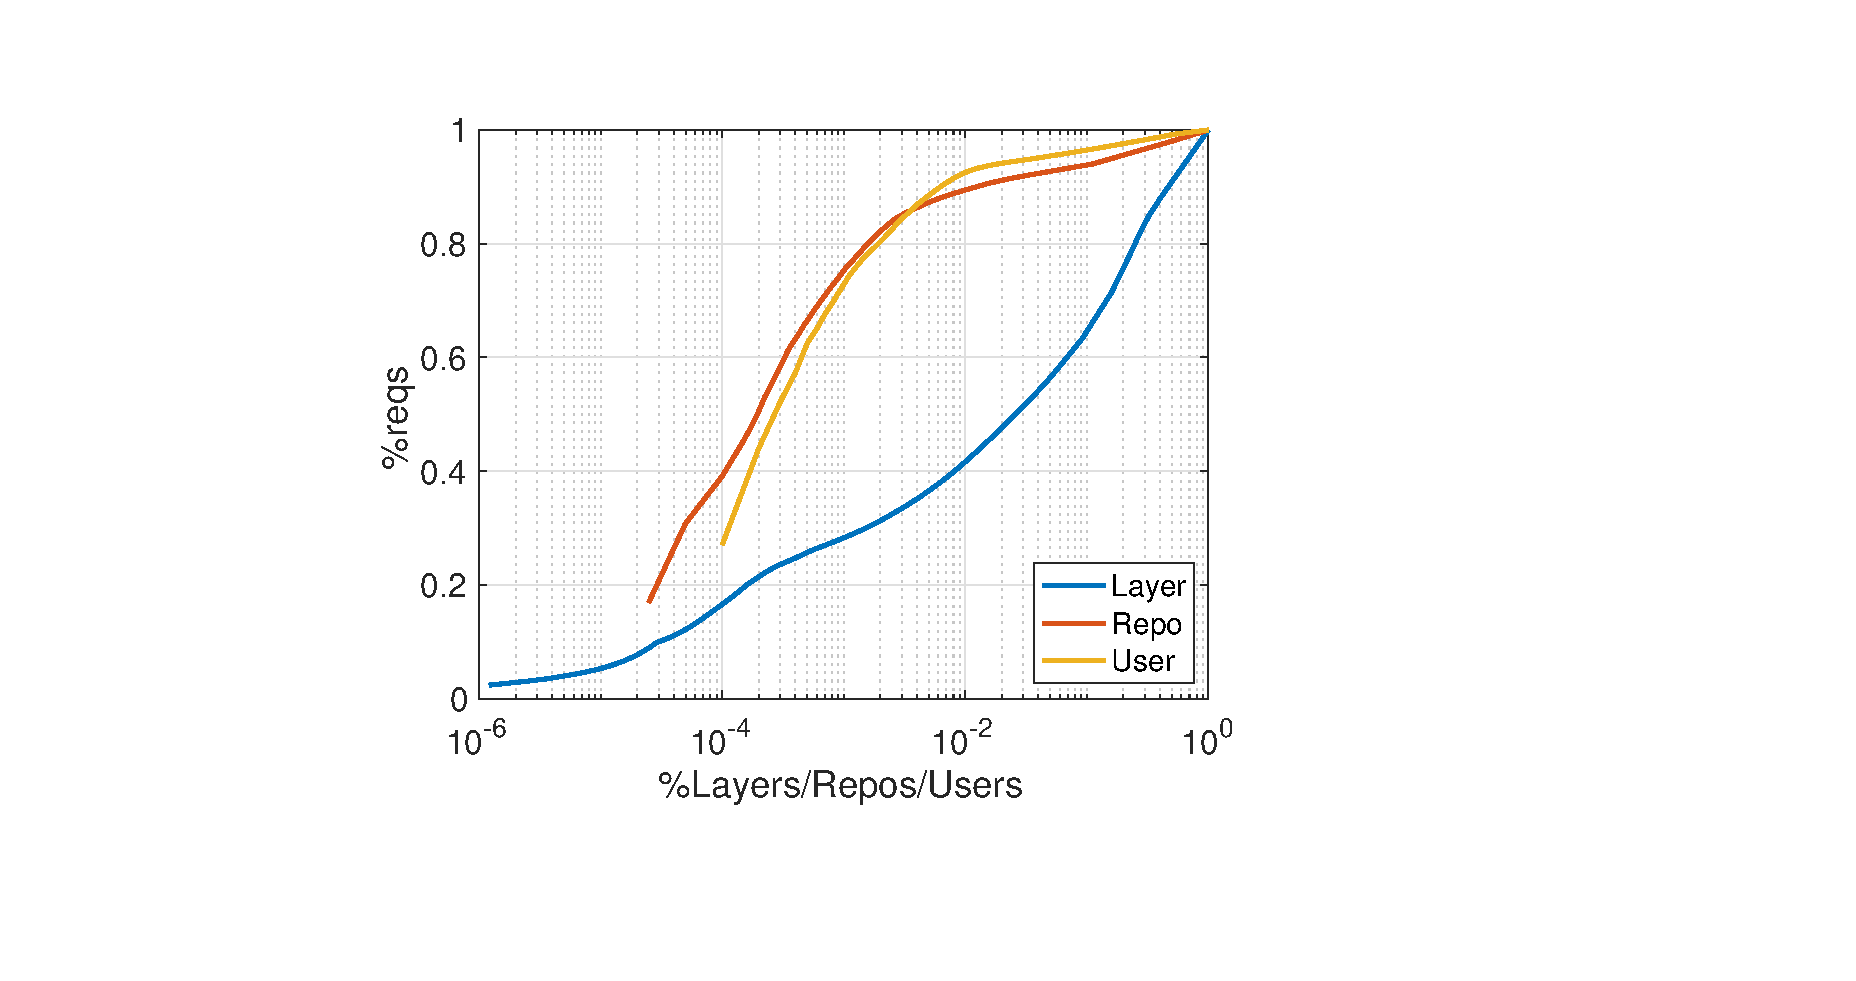
\includegraphics[width=1\textwidth]{graphs/skewness_cdf.eps}
			\caption{Popularity of layers, repos, and users.}
			\label{fig:sknewss}
		\end{minipage}
	\begin{minipage}{0.225\textwidth}
		\centering
		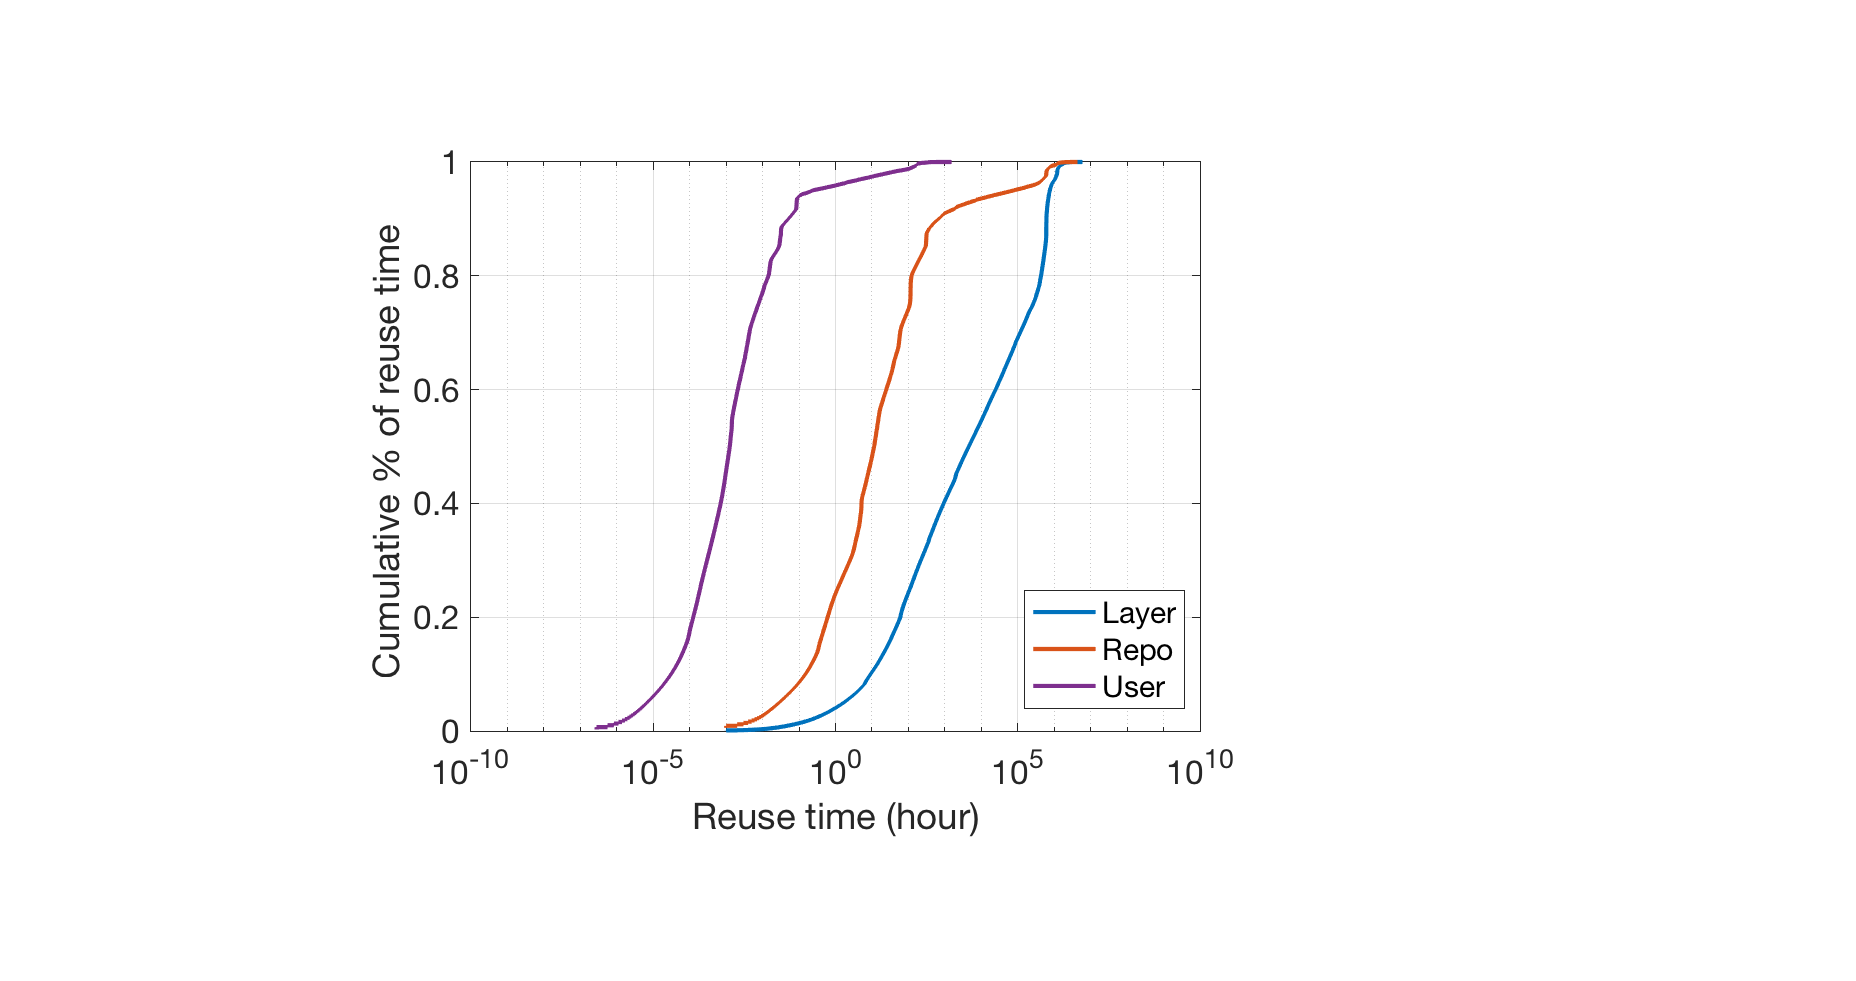
\includegraphics[width=1\textwidth]{graphs/reuse_time.eps}
		\caption{CDF of reuse time for layers, repos, and users.}
		\vspace{-3pt}
		\label{fig:reusetime}
	\end{minipage}
\end{figure}

\paragraph{Understanding layer access patterns.}
We analyzed the Dallas(\texttt{dal}) registry workload collected from IBM Container Registry over the course of 75 days~\cite{dockerworkload}. 
Figure~\ref{fig:sknewss} shows the registry accesses to layers and repositories, as well as users accesses to the layers and manifests.
% \arb{layers??}\NZ{addressed}. 
Layer accesses are heavily skewed. For example, $25$\% of popular layers account for $80$\% of all requests. 
For repository accesses and accesses by users, the skew is more significant than it is for layers. %10\% most frequently accessed repositories account for 94\% of all requests
$94$\% of all requests accessed only $10$\% of the (popular) repositories. Similarly, only $9$\% of (most active) users issued $97$\% of all requests. 
This means that only a few extremely active users create their repositories in the \texttt{dal} registry and issue the majority of requests to the registry.

Figure~\ref{fig:reusetime} shows the reuse time of layers and repositories and users.
Layer reuse time is the duration between two consecutive requests to the same layer or repository. Similarly,
reuse time by user is duration between two consecutive same-user requests.
The layer reuse time is long.
The median reuse time of a layer is $1.3$ hours. $80$\% of repositories experience the highest request frequency, with a reuse time of $2$ minutes. 
$90$\% of users remain active for at least $0.06$ seconds, thus most layers are not requested within a short time period.
%So for a registry, most of its stored layers are not accessed frequently given a very short time period while
%users can maintain active for a longer time. 
%This is because users can access multiple layers and manifests.
%   Thus, most of the layers stored in the
%   registry are not frequently requested over very short
%   time periods.
%, while users remain active for a longer time.
%This is because users can request different layers or manifests.

To quantify the efficacy of traditional LRU and push-pull prefetching,
we implemented an LRU algorithm and push-pull prefetching~\cite{dockerworkload} 
and replayed 
IBM registry workload \texttt{dal} with different cache size as shown in 
Figure~\ref{fig:lru_prefetching_hits}.
The hit ratio for LRU was found to be lower than $60$\% across different sizes.
This is because layer accesses do not follow LRU temporal trend:
recently pulled layer will not be pulled again by the same user.
Although push-pull prefetching slightly improved the hit ratio compared to LRU,
the maximum hit ratio is still low and stays stable around $80$\%.
This is because push-pull prefetching predicts the future accesses based on  
pushed layers.
However, based on our above trace analysis,
only half of the \texttt{pull} layer
requests have a preceding \texttt{push} layer request within the trace
%collecting duration
collection period of 75 days. This means that, after a user pushes a layer
to the registry, it takes a few days, weeks, or even months for a user to make
a \texttt{pull} request. 
%Second, we found in the traces only half of the pull layer requests have a preceding 
%push layer request and push-pull prefetching ignored the layers that were pushed 
%before data collection.

%Anwar et
%al. have proposed a prefetching method~\cite{dockerworkload} based on the
%\texttt{push}-\texttt{pull} relationship: whenever there is a \texttt{PUSH} layer
%request directly followed by a \texttt{GET} manifest request, with a high probability these will be followed by a \texttt{GET}
%layer request.


%\arb{say something whether this is good or bad... or is very low and show that LRU is not an effective mechanism for managing the proposed caches}\NZ{addressed}

\paragraph{Registry as a cache for improving performance.}
Traditionally, caches are placed as close to the requesting client as 
proxy caches, or web/HTTP caches for the temporary storage of 
frequently requested data to mitigate the remote server lag. 
For example, Varnish~\cite{varnish} and Squid~\cite{squid} are high-performance web/HTTP caches that accelerate web applications and improve response times by caching frequently requested web content.
%Examples of open-source web (HTTP) proxy caches include Nginx~\cite{?}, Squid~\cite{?}, and Varnish~\cite{?}. 
%They are typically implemented in an regional ISP or within a corporate network.
%Deduplication methods are implemented on remote backend storage servers, and
%transparently remove duplicates from the incoming data stream and restore the data for read requests. 
Docker registry is a web server that serves docker \texttt{pull} and docker \texttt{push} requests.
Intuitively, registries can be deployed as proxy caches, \ie a pull-through cache~\cite{registryascache}, to host frequently requested layers. This will speedup image pulls and improve performance. 

However, the layer access pattern differs greatly from traditional request streams.
Traditional LRU will place recently requested data into the cache 
because it is highly likely that the data will be requested again.
However, it is the opposite for the layer access pattern: if a layer is pulled by a user,
then this layer will not be pulled by the same user in the future
since the layer is now locally available to the user. Thus, we have to design innovative mechanisms to manage any caches.



%We analyzed IBM registry workload and made the two following obervations:
%Caching is a technique widely leveraged to reduce bandwidth and load off of highly loaded bottleneck backends by temporarily storing frequently requested data~\cite{xxx}. 
%Caching can be introduced at the client, in between clients and servers as a proxy, or at the server side. 
%Proxy caches are efficient in reducing traffic from bottleneck backends by cooperatively serving previously requested and saved data without it going all they way to the backend~\cite{xxxx}. 
%Usually, caches are placed as close to the requesting client as possible, 
%such caches are known as proxy caches, or web/HTTP caches for the short-lived storage of 
%frequently requested/accessed data to reduce the server's lag. 

%The client therefore, experiences improved response times.
%The Docker client inherently caches layers at the client. This way, the Docker daemon only pulls layers that are not available on the host machine. 

%Other software used for caching include Memcached~\cite{?}, an open-source distributed in-memory key-value store that works as a caching system and Redis~\cite{?} which is an open-source key-value store that works as an in-memory store and as a cache
%\subsection{Apply traditional deduplication approaches to registries?}
%\subsection{Use-cases of \sysname}
%This suggests that the current layer sharing strategy that Docker already employs is not efficient in eliminating duplicate data. 
%Further investigations on the causes for the high number of redundant files exposed a few findings. 
%For example, different Docker images often contain the same 
%source code from external public repositories like GitHub~\cite{github}.
%This is because no official images contain this source code, 
%so users manually add it to their images, 
%resulting in different layers which cannot be reused.
%\paragraph{Deduplication statistics} % the potential of deduplication 

%%%%layer ref count 
%
%A remarkable observation that emerges from the data analysis is that only around 3\%\HA{3\% or 7\% ?} of the layers' constituent files are unique while the rest are redundant copies. 
%This suggests that the current layer sharing strategy that Docker already employs is not efficient in eliminating duplicate data. 
%We further analyzed the repeat count for every file and plotted the distributions as shown in Figure~\ref{fig:file-repeat-cnt}.
%We found that over 99.4\% of files have more than one copy.
%Around 50\% of files have exactly 4 copies and 90\% of files have 10 or less copies. 
%This indicates the high potential for file-level deduplication in the Docker registry.
%
%\begin{figure} \centering
	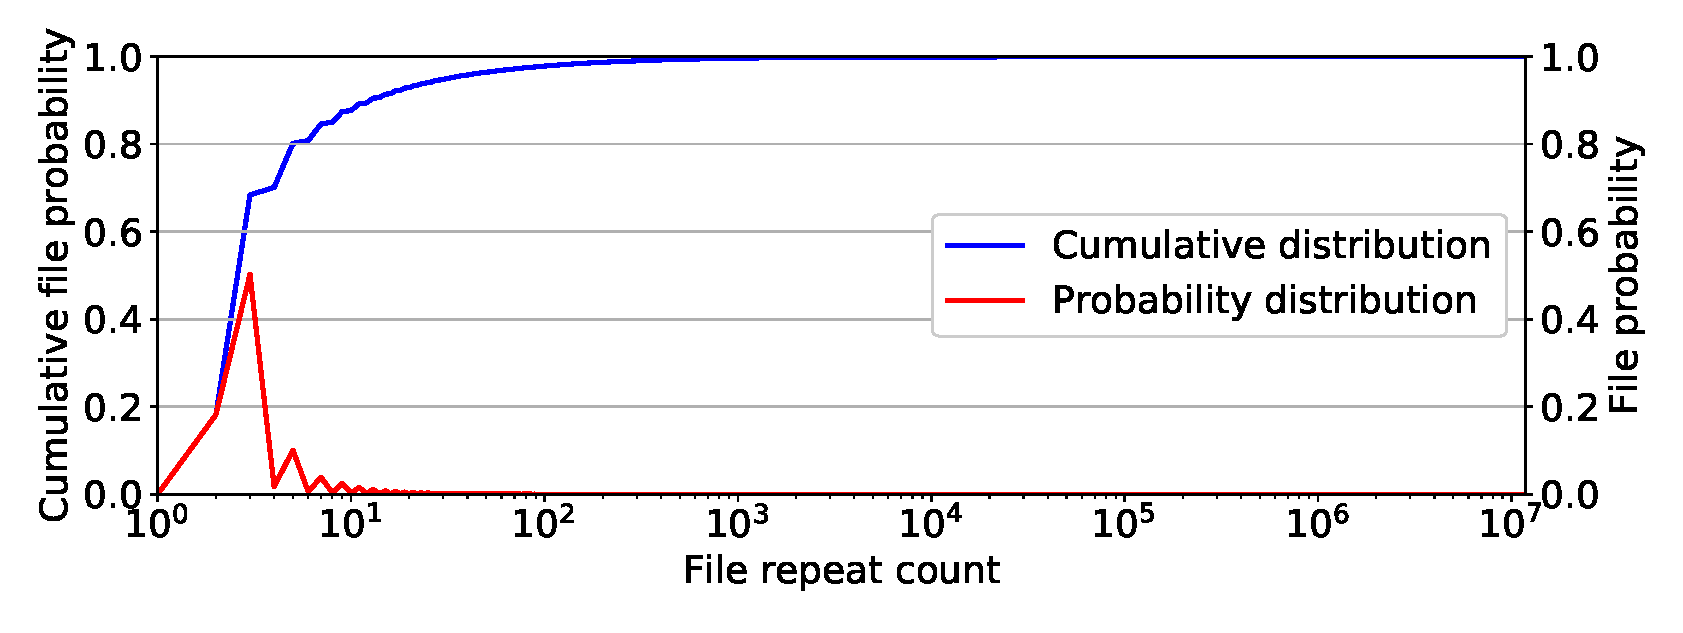
\includegraphics[width=0.45\textwidth]{graphs/File_repeat_count.eps}
	\caption{File repeat count distribution.
	%
	\VT{No need for Y2}
	%
	\VT{Still need to use \% on the axis}
	%
	} \label{fig:file-repeat-cnt}
\end{figure}

%
%
%\paragraph{Deduplication ratio growth} % benefit
%%
%Further investigations on the potential of file-level deduplication involved analyzing the deduplication ratio. 
%As shown in Figure~\ref{fig:dedup-ratio-growth}, we analyzed the deduplication 
%ratio and its growth for an increasing number of files stored in the registry.   
%%(see Figure~\ref{fig:dedup-ratio-growth}).
%%
%%Figure~\ref{fig:dedup-ratio-growth} shows the deduplication ratio growth over the layer dataset size. 
%%
%The x-axis values correspond to the sizes of 4 random samples drawn from the whole dataset and the size of the
%whole dataset.
%
%We see that the deduplication ratio increases almost linearly with the layer dataset size.
%This implies that the benefits of file-level deduplication strengthens as the number of public repositories and images grow.
%
%As the number of images stored in the Docker registry increases dramatically,
%file-level deduplication can provide significant storage space savings.

%Intuitively, registries can be deployed as a proxy cache to host frequently requested layers to speedup image pulls and improve performance 
%while the backend cloud storage can leverage deduplication to save storage space.
%However, there are several unique problems concerning the integration of caching and deduplication to the unique Docker registries workload: \textbf{compressed layers}. 

%\subsection{Need for Usr-oriented cache management}
%
%\paragraph{Access skewness}
%
%\paragraph{Reuse time distribution}
%
%\paragraph{Hit ratios}
%
%\paragraph{Hit ratios with prefetching}
%
%%\subsection{} % what are the cost for a naive file-level deduplication
%
%\paragraph{Restoring performance breakdown}


